% !TEX spellcheck = en_US
% !TEX encoding = UTF-8

\documentclass[xcolor={x11names, table}, compress]{beamer}

  \usepackage{xcolor}
  \usepackage{fontspec}
  \usepackage{pgfplots}
  \usepackage{tikz}
  \usepackage{amsmath, amssymb, amsfonts}
  \usepackage{bm}
  \usepackage{eso-pic}
  \usepackage{graphicx}
  \usepackage{verbatim}
  \usepackage[backend=biber]{biblatex}
  
  \pgfplotsset{compat=1.15}
  \usetikzlibrary{positioning, shapes, calc, arrows}
  \hypersetup{pdfstartview={Fit}}
  
  %% Beamer Layout %%%%%%%%%%%%%%%%%%%%%%%%%%%%%%%%%%
  \useinnertheme{default}
  \usepackage[T1]{fontenc}
  \usefonttheme{professionalfonts}
  
  \setbeamerfont{frametitle}{}
  
  \definecolor{BHKpresentationDark}{RGB}{114,133,176}
  \definecolor{BHKpresentationDarkGrey}{RGB}{103,116,128}
  \definecolor{BHKblue}{RGB}{51,105,153}
  
  \setbeamerfont{title like}{shape=\scshape}
  \setbeamercolor*{frametitle}{fg=BHKpresentationDark} 
  \setbeamercolor*{lower separation line head}{bg=BHKblue} 
  \setbeamercolor*{normal text}{fg=BHKpresentationDarkGrey,bg=white} 
  \setbeamercolor*{alerted text}{fg=BHKblue} 
  \setbeamercolor*{example text}{fg=black} 
  \setbeamercolor*{item}{fg=BHKpresentationDark,bg=gray} 
  \setbeamercolor{enumerate item}{fg=BHKpresentationDark}
  \setbeamercolor*{structure}{fg=black} 
  \setbeamercolor*{palette tertiary}{fg=black,bg=black!10} 
  \setbeamercolor*{palette quaternary}{fg=black,bg=black!10} 
  \setbeamercovered{transparent}
  
  \setbeamertemplate{navigation symbols}{}
  \setbeamertemplate{footline}{%
      \begin{beamercolorbox}[wd=\paperwidth]{footlinecolor}
          \includegraphics[width=\textwidth]{bar_footline.pdf}
      \end{beamercolorbox}%
  }
  
  \setbeamertemplate{frametitle}[default][center]
  \setbeamertemplate{caption}[numbered]
  \setbeamertemplate{section in toc}[sections numbered]
  \setbeamertemplate{subsection in toc}[subsections numbered]
  
  
  \newcommand{\insertsec}{\thesection.~\insertsection}
  \newcommand{\insertsubsec}{\thesection.\thesubsection~\insertsubsection}
  
  %%%%%%%%%%%%%%%%%%%%%%%%%%%%%%%%%%%
  %% Start of document %%%%%%%%%%%%%%
  %%%%%%%%%%%%%%%%%%%%%%%%%%%%%%%%%%%
  
  \begin{document}
  %%%% title slide %%%%%
  {\setbeamertemplate{footline}{} 
      \begin{frame}
          \vspace{-1.5cm}
          \hfill\makebox[0.2\paperwidth]{\includegraphics[width=0.4\textwidth]{logo_wtext}}
          \begin{flushleft}
              \hspace{-1cm}\includegraphics[width=0.8\textwidth, height=0.4em]{title_line.pdf}\hfill
              
              \title{
                  \begin{flushleft}{\huge \color{BHKpresentationDark} 
                  Convolutional Neural Networks Summary
              } 
              \end{flushleft}}
              
              \date{$~~$}
              \author[Joan]{\begin{flushleft}\vspace{-1cm} Joan Marcè i Igual\end{flushleft}}
              \titlepage
          \end{flushleft}
      \end{frame}
  }
  
  \begin{frame}{Table of Contents}
    \tableofcontents
  \end{frame}
  
  % !TEX root = ../main.tex

\section{Introduction}
\begin{frame}{\insertsec}
	\begin{itemize}
    \item Nowadays Machine Learning is widely used
    \item Medical images can be obtained using MRI, PET or CT scans but are underused
    \item Different methods have appeared to analyze these data for image classification,
    object detection, segmentation...
    \item Deep learning models aim to be able to unlock the full potential of medical imaging
    \item Hand-crafted radiomic features can be extracted from medical images
  \end{itemize}
\end{frame}

\subsection{Survival Analysis}
\begin{frame}{\insertsubsec}
  Survival analysis models usually have:
  \begin{itemize}
    \item Baseline data \( x \)
    \item Event \( E \in \{0, 1\} \)
    \item Time \( T \)
  \end{itemize}
  
  Survival function:
  \[
    S(t) = \Pr(T \ge t)
  \]

  Hazard function:
  \[
    \lambda(t) = \lim_{\Delta t \rightarrow 0}
    \frac{\Pr(t \le T < t + \Delta t | T \ge t)}{\Delta t}
  \]
\end{frame}

\begin{frame}

  Casting the survival problem as a ranking is a way of dealing with censored data.

  \begin{columns}
    \begin{column}{.5\textwidth}
      \begin{figure}
        \centering
        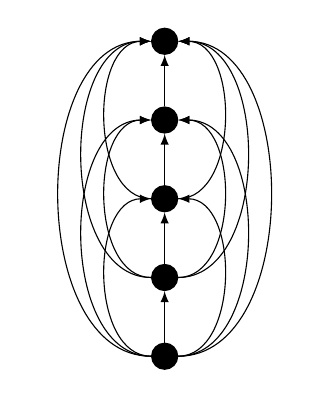
\begin{tikzpicture}
  \tikzstyle{bDot}=[circle, fill=black, draw]
  \foreach \y in {1,...,5} {
    \node[bDot] (D-\y) at (0, \y) {};
  }

  \foreach \y in {1,...,4} {
    \pgfmathsetmacro{\z}{int(\y + 1)}
    \draw[-latex] (D-\y) -- ({D-\z}.south);
  }

  \foreach \y in {1,...,3} {
    \pgfmathsetmacro{\z}{int(\y + 2)}
    \foreach \j in {\z,...,5} {
      \ifthenelse{\y=2 \OR \y=3}{
        \draw[-latex] (D-\y) to[bend left=90] (D-\j);
      }{
        \draw[-latex] (D-\y) to[bend right=90] (D-\j);
      }
    }
  }
\end{tikzpicture}

        \caption{Uncensored data}
      \end{figure}
    \end{column}
    \begin{column}{.5\textwidth}
      \begin{figure}
        \centering
        \begin{tikzpicture}
  \foreach \y in {1,...,5} {
    \ifthenelse{\y=2 \OR \y=4}{
      \node [circle, fill=white, draw=black] (D-\y) at (0, \y) {};
    }{
      \node [circle, fill=black, draw=black] (D-\y) at (0, \y) {};
    }

    \foreach \y in {3,4,5} {
      \draw [-latex] (D-1) to[bend right=90] (D-\y);
    }

    \foreach \y/\z in {1/2, 3/4} {
      \draw [-latex] (D-\y) -- (D-\z);
    }
    \draw [-latex] (D-3) to[bend left=90] (D-5);
  }
\end{tikzpicture}

        \caption{Censored data}
      \end{figure}
    \end{column}
  \end{columns}
\end{frame}

\begin{frame}
  \begin{itemize}
    \item Both of them are uncensored (\( \bm{E}_i = \bm{E}_j = 1\))
    \item The uncensored time of one is smaller than the censored survival time of the other
    (\( \bm{T}_i < \bm{T}_j | \bm{E}_i = 1; \bm{E}_j = 0 \))
  \end{itemize}

  Concordance Index:
  \[
    CI = \frac{\text{Good predictions}}{\text{Total predictions}} \in [0, 1]
  \]
\end{frame}
 
  % \section{Neural Networks}
\begin{frame}{\insertsec}
	\def\layersep{2.5cm}

\begin{figure}[H]
    \centering
    \begin{tikzpicture}[shorten >=1pt,->,draw=black!50, node distance=\layersep]
        \tikzstyle{every pin edge}=[<-,shorten <=1pt]
        \tikzstyle{neuron}=[circle,fill=black!25,minimum size=17pt,inner sep=1pt]
        \tikzstyle{input neuron}=[neuron, fill=green!50];
        \tikzstyle{output neuron}=[neuron, fill=red!50];
        \tikzstyle{hidden neuron}=[neuron, fill=cyan!50];
        \tikzstyle{annot} = [text width=4em, text centered]
        
        % Draw the input layer nodes
        \foreach \y in {1,...,4} {
            % This is the same as writing \foreach \name / \y in {1/1,2/2,3/3,4/4}
            \node[input neuron] (I-\y) at (0,-\y) {$x^{(\y)}$};
        }
        % Draw the hidden layer nodes
        \foreach \y in {1,...,5} {
            \node[hidden neuron, yshift=.5cm] (H-\y) at (\layersep,-\y cm) {$a^{(\y)}$};
        }
        
        % Draw the output layer node
        \node[output neuron,pin={[pin edge={->}]right:Output}, right of=H-3] (O) {};
        
        % Connect every node in the input layer with every node in the
        % hidden layer.
        \foreach \source in {1,...,4}
            \foreach \dest in {1,...,5}
                \path (I-\source) edge (H-\dest);
        
        \path (I-1) edge node[sloped, above] {\footnotesize  $w_{1, 1}^{[1]}$} (H-1);
        
        % Connect every node in the hidden layer with the output layer
        \foreach \source in {1,...,5}
            \path (H-\source) edge (O);
        
        % Annotate the layers
        \node[annot,above of=H-1, node distance=1cm] (hl) {Hidden layer};
        \node[annot,left of=hl] {Input layer};
        \node[annot,right of=hl] {Output layer};
    \end{tikzpicture}
    \caption{Representation of Neural Network}
\end{figure}

\end{frame}

\subsection{Parameters}
\begin{frame}{\insertsubsec}
    \begin{columns}[t]
        \column{.6\textwidth}
        \begin{itemize}
            \item $l$: Current layer
            \item $w_{i, j}^{[l]}$: Weight from unit $j$ to $i$ at layer $l$
            \item $b_{i}^{[l]}$: Bias for unit $i$ at layer $l$
            \item $n^{[l]}$: Number of units in layer $l$
            \item $W^{[l]} \in \mathbb{R}^{n^{[l]} \times n^{[l - 1]}}$: Weight matrix
            \item $\bm{b}^{[l]} \in \mathbb{R}^{n^{[l]}}$: Bias
            \item $
            \begin{aligned}[t]
                \bm{a}^{[l]} &= g(W^{[l]}\cdot \bm{a}^{[l - 1]} + \bm{b}^{[l]}) \\
                \bm{a}^{[l]} &\in \mathbb{R}^{n^{[l]}}
            \end{aligned}
            $ Activations for layer $l$
            \item $g(x)$: Activation function
        \end{itemize}
        \column{.5\textwidth}
        \centering
        \begin{columns}[t]
    \column{.5\textwidth}
    \centering
    \begin{figure}
        \begin{tikzpicture}
            \begin{axis}[
                width=\textwidth,
                height=.8\textwidth,
                grid=major,
                grid style={dashed, gray!30},
                xtick={-5, 0, 5},
                xticklabels={$-\infty$, $0$, $+\infty$}
                ]
                \addplot[mark=none]{tanh(x)};
            \end{axis}
        \end{tikzpicture}
        \caption{$\tanh(x)$}
    \end{figure}
    \centering
    \column{.5\textwidth}
    \begin{figure}
        \begin{tikzpicture}
            \begin{axis}[
                width=\textwidth,
                height=.8\textwidth,
                grid=major,
                grid style={dashed, gray!30},
                xtick={-5, 0, 5},
                xticklabels={\empty, $0$, \empty}
                ]
                \addplot[mark=none]{max(x, 0)};
            \end{axis}
        \end{tikzpicture}
        \caption{ReLU function}
    \end{figure}
\end{columns}
    \end{columns}
\end{frame}
\begin{frame}
    \begin{columns}
        \column{.6\textwidth}
        \begin{block}{Cost function}
            $$
            J(\bm{W}, \bm{b}, \hat{\bm{y}}, \bm{y}) = 
            \frac{1}{m} \sum_{i=1}^{m} \mathcal{L}(\hat{\bm{y}}^{(i)}, \bm{y}^{(i)})
            $$
        \end{block}
        \begin{block}{Loss function}
            $$
            \mathcal{L}(\hat{\bm{y}}, \bm{y}) = ||\hat{\bm{y}} - \bm{y}||^2
            $$
        \end{block}
        \begin{block}{Parameters update}
            \begin{align*}
            W^{[l]} &:= W^{[l]} - \alpha \cdot \frac{\partial J}{\partial W^{[l]}} \\
            \bm{b}^{[l]} &:= \bm{b}^{[l]} - \alpha \cdot \frac{\partial J}{\partial \bm{b}^{[l]}}
            \end{align*}
        \end{block}
        \column{.4\textwidth}
        To achieve better results at predicting $\hat{\bm{y}}$ 
        we have to minimize the cost function $J(\bm{W}, \bm{b}, \hat{\bm{y}}, \bm{y})$.
    \end{columns}
\end{frame}

\subsection{Regularization}
\begin{frame}{\insertsubsec}
    To prevent overfitting add the weights to the cost function so we also try to minimize
    big weights.

    \begin{align*}
        J(\bm{W}, \bm{b}, \hat{\bm{y}}, \bm{y}) &= 
        \frac{1}{m} \sum_{i = 1}^m \mathcal{L}(\hat{\bm{y}}, \bm{y}) + 
        \frac{\lambda}{2m} \sum_{l=1}^L ||W^{[l]}||^2_F \\ 
        \underbrace{||W^{[l]}||^2_F}_{\text{Frobenius Norm}} &= \sum_i \sum_j (w_{ij}^{[l]}) \\ 
        dW^{[l]} &= \text{from backprop } + \frac{\lambda}{m} \cdot W^{[l]} \\
        \lambda &\rightarrow \text{Regularization parameter}
    \end{align*}

    It cancels some effects from some units creating a simple model.
\end{frame}
\begin{frame}[fragile]{Dropout Regularization}
    Go through each layer of the network and set some probability of elimination for each unit. 
    This is done for \textbf{each sample}.

    \begin{figure}
        \begin{verbatim}
drop = np.random.randn(*a_prev.shape) < keep_prob
a_next = np.multiply(a_prev, drop)
a_next /= keep_prob
        \end{verbatim}
        \caption{Example using \texttt{numpy}}
    \end{figure}

    \begin{alertblock}{Predictions during test time}
        No dropout is used during test time since it wouldn't make sense.
    \end{alertblock}
\end{frame}

\begin{frame}{Adam optimization algorithm}
    Training a NN is a minimization problem. In this case we always use gradient descent
    to find the minimum. Sometimes the gradient can go too fast.

    \begin{onlyenv}<1>
        \begin{align*}
            V_{dW} &= \beta_1 V_{dW} + (1 - \beta_1) \cdot dW \\
            S_{dW} &= \beta_2 S_{dW} + (1 - \beta_2) \cdot dW^2 \\
            W &:= W - \alpha \cdot \frac{V_{dW}}{\sqrt{S_{dW}} + \varepsilon}
        \end{align*}
    \end{onlyenv}
    \begin{onlyenv}<2>
        
\begin{figure}[H]
    \begin{tikzpicture}
\begin{axis}[
        width=.9\textwidth,
        height=.6\textwidth,
        xlabel=Day,
        ylabel={T $(^{\circ}C)$},
        every axis y label/.style={at={(current axis.north west)},above=2mm},
        ymax = 45,legend style={font=\fontsize{4}{5}\selectfont},
        clip marker paths=true
    ]
    \addplot[
        mark=*,
        mark size=1,
        draw=cyan!50
    ] table[
        x index = 0, 
        y index = 1, 
        header=true, 
        col sep = comma, 
        only marks
    ]{drawings/daily_temperature.csv};
    \addlegendentry{Data}
    \addplot[
        mark=none,
        draw=red!50,
        thick
    ] table[
        x index = 0, 
        y index = 2, 
        header=true, 
        col sep = comma
    ]{drawings/daily_temperature.csv};
    \addlegendentry{$\beta = .99$}
    \addplot[
        mark=none,
        draw=violet,
        thick
    ] table[
        x index = 0, 
        y index = 4, 
        header=true, 
        col sep = comma
    ]{drawings/daily_temperature.csv};
    \addlegendentry{$\beta = .90$}
\end{axis}
    \end{tikzpicture}
    
\end{figure}



    \end{onlyenv}
\end{frame}

\subsection{Hyper-parameters}
\begin{frame}{\insertsubsec}
    \begin{itemize}
        \item $m$: Mini-batch size
        \begin{itemize}
            \item $m = 1$: Stochastic gradient descent
            \item $m = $ set size: Batch gradient descent
        \end{itemize}
        \item $\alpha$: Learning rate
        \begin{itemize}
            \item Learning rate decay 
            $\alpha = \frac{1}{1 + \text{decay-rate}\times \text{epoch}} \cdot \alpha_0$
            \item Exponential decay
            $\alpha = 0.95^{\alpha_0}$

        \end{itemize}
        \item $L$: Number of layers
        \item Number of iterations
        \item Number of hidden units
    \end{itemize}
\end{frame}

  % \section{Convolutional Neural Networks}
\begin{frame}{\insertsec}
    This type of networks are a bit different because instead of computing the activations by
    multiplying the previous ones with the weight matrix it convolutes the previous activations 
    (denoted by $*$):
    
    \begin{align*}
        \bm{a}^{[l]} &= g(\bm{W}^{[l]}\cdot \bm{a}^{[l - 1]} + \bm{b}^{[l]}) \\
        \text{Becomes:} \\
        \bm{a}^{[l]} &= g(\bm{W}^{[l]} * \bm{a}^{[l-1]} + \bm{b}^{[l]})
    \end{align*}
\end{frame}

\subsection{Convolution Operation}
\begin{frame}{\insertsubsec}
    \begin{alertblock}{Important}
        What we call \textit{Convolution} in ML it's actually the \textit{Cross-Correlation} operation
        in signal analysis.
    \end{alertblock}
    
    \begin{align*}
        \left(
        \begin{array}{cccccc}
            10 & \cellcolor{green!20}10 & \cellcolor{green!20}10 & \cellcolor{green!20}0 & 0 & 0 \\
            10 & \cellcolor{green!20}10 & \cellcolor{green!20}10 & \cellcolor{green!20}0 & 0 & 0 \\
            10 & \cellcolor{green!20}10 & \cellcolor{green!20}10 & \cellcolor{green!20}0 & 0 & 0 \\
            10 & 10 & 10 & 0 & 0 & 0 \\
            10 & 10 & 10 & 0 & 0 & 0 \\
            10 & 10 & 10 & 0 & 0 & 0 \\
        \end{array}
        \right)
        *
        \left(
        \begin{array}{ccc}
            1 & 0 & -1 \\
            1 & 0 & -1 \\ 
            1 & 0 & -1 \\
        \end{array}
        \right)
        = 
        \left(
        \begin{array}{cccc}
            0 & \cellcolor{green!20}30 & 30 & 0 \\
            0 & 30 & 30 & 0 \\
            0 & 30 & 30 & 0 \\
            0 & 30 & 30 & 0 \\
        \end{array}
        \right)
    \end{align*}
    $$
        10 \cdot 1 + 10 \cdot 1 + 10 \cdot 1 +
        10 \cdot 0 + 10 \cdot 0 + 10 \cdot 0 +
        0 \cdot -1 + 0 \cdot -1 + 0 \cdot -1 = 30
    $$
\end{frame}

\subsection{Pooling operation}
\begin{frame}{\insertsubsec}
    We use pooling to reduce the volume width and height size
    \begin{block}{Max-Pooling}
        \begin{align*}
            \operatorname{max\,pool}
            \left(
            \begin{array}{cccc}
                \cellcolor{green!20} 0 & \cellcolor{green!20} 7 & 12 &  9 \\
                \cellcolor{green!20}15 & \cellcolor{green!20} 3 & 22 &  6 \\
                 2 & 12 &  8 &  3 \\
                 6 &  2 & 18 &  3 \\
            \end{array}
            \right)
            =
            \left(
            \begin{array}{cc}
                \cellcolor{green!20}15 & 22 \\
                12 & 18
            \end{array}
            \right)
        \end{align*}
    \end{block}

    \begin{block}{Avg-Pooling}
        \begin{align*}
            \operatorname{avg\,pool}
            \left(
            \begin{array}{cccc}
                \cellcolor{green!20} 0 & \cellcolor{green!20} 7 & 12 &  9 \\
                \cellcolor{green!20}15 & \cellcolor{green!20} 3 & 22 &  6 \\
                 2 & 12 &  8 &  3 \\
                 6 &  2 & 18 &  3 \\
            \end{array}
            \right)
            =
            \left(
            \begin{array}{cc}
                \cellcolor{green!20}6.25 & 12.25 \\
                5.50 & 8.00
            \end{array}
            \right)
        \end{align*}
    \end{block}
\end{frame}

\subsection{Residual Networks}
\begin{frame}{\insertsubsec}
    They are a type of network that can learn the identity function thus allowing us to do
    very deep networks.
    \def\layersep{1.5cm}

\begin{figure}[H]
    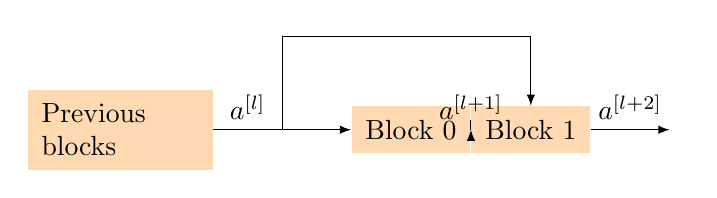
\begin{tikzpicture}[node distance=\layersep]
        \tikzstyle{block}=[rectangle, fill=orange!30, inner sep = 5pt]
        \node[block] (R0) at (0, 0) {Block 0};
        \node[left = .75 of R0] (A0) {};
        \node[above = .75 of R0] (A1) {};
        \node[block, left = .75 of A0, text width = 2cm] (I0) {Previous blocks};
        \node[block, right = of R0] (R1) {Block 1};
        \node[right = 1 of R1] (A2) {};

        % Arrows
        \draw [-latex] (I0) -- (R0) node[above, near start] {$a^{[l]}$};
        \draw [-latex] (R0) -- (R1) node[above, midway] {$a^{[l + 1]}$};
        \draw (A0.center) |- (A1.center); 
        \draw [-latex] (A1.center) -| (R1.north);
        \draw [-latex] (R1) -- (A2) node[above, midway] {$a^{[l + 2]}$};
    \end{tikzpicture}
\end{figure}

    \begin{align*}
        \bm{a}^{[l+2]} = 
        g(\underbrace{W^{[l+2]} \cdot \bm{a}^{[l + 1]} + \bm{b}^{[l + 2]}}
        _{0 \text{ if using regularization}} + \bm{a}^{[l]})
    \end{align*}
\end{frame}
  
  
  
  \end{document}